\documentclass{article}

\usepackage[dblblindworkshop]{neurips_2026}
\workshoptitle{New In Machine Learning (NewInML)}

\usepackage[utf8]{inputenc}
\usepackage[T1]{fontenc}
\usepackage{amsmath,amssymb,amsthm,mathtools}
\usepackage{booktabs}
\usepackage{graphicx}
\usepackage{microtype}
\usepackage{xcolor}
\usepackage{url}
\usepackage{hyperref}
\hypersetup{hidelinks}

\newtheorem{theorem}{Theorem}
\newtheorem{corollary}{Corollary}
\DeclareMathOperator*{\argmin}{arg\,min}
\DeclareMathOperator*{\argmax}{arg\,max}
\newcommand{\M}{\mathcal{M}}
\newcommand{\Q}{\mathcal{Q}}
\newcommand{\E}{\mathcal{E}}
\newcommand{\RRlo}{\underline{\Gamma}}
\newcommand{\RRhi}{\overline{\Gamma}}

% Result macros are populated only from frozen, content-addressed result files.
\newcommand{\CoverageResult}{HRMS achieved 95.8--98.6\% joint coverage across latent-Gaussian ICC $0$--$.5$, versus 70.2--77.6\% for fixed-denominator max-$t$, while pairing made its intervals 51--52\% narrower than conservative simultaneous separate-risk bounds}
\newcommand{\RegretResult}{HRMS matched the 500,000-draw reference-population robust optimum and reduced robust regret by 36.2\% relative to the uniform-environment mean at the strongest simulated reversal; point robust-regret selection also matched the optimum}
\newcommand{\CivilResult}{the nominal 95\% set excluded none of $12$ candidates, and its minimum-upper-bound default did not minimize realized test robust regret; an IID-root sensitivity analysis changed that forced point choice}
\newcommand{\CivilObservations}{12,823/37,226}
\newcommand{\CivilRoots}{3,046/8,792}
\newcommand{\CivilCandidates}{12}

\title{Reliable Model Selection Under Hierarchical Dependence and Unknown Environment Mixtures}
\author{Anonymous authors}

\begin{document}
\maketitle

\begin{abstract}
Model selection under distribution shift often relies on correlated, multi-environment validation data.  We introduce Hierarchical Robust Model Selection (HRMS), which constructs paired root-cluster-aware simultaneous risk-difference bounds, propagates them to worst-case regret over plausible mixtures of represented environments, and returns a confidence set when a unique robust optimum is unsupported.  Joint pairwise coverage deterministically transfers to regret and set coverage; simulations assess bootstrap calibration.  Pairing narrows near-nominal simulated bounds, and robust selection improves on nominal averaging under severe rank reversal.  On a public homology-controlled TE--cCRE benchmark, four TE families have different test winners and HRMS gives a radius-stable default, yet its default-radius 95\% set retains all 24 candidates.  A derived CivilComments study likewise retains all 12: a forced operational default can coexist with inferential non-uniqueness.
\end{abstract}

\section{Introduction}
\label{sec:intro}

Choosing a deployable model is not the same problem as training one.  Suppose a practitioner has a frozen library of trained candidates and a validation table containing every candidate's prediction on every record.  Three complications commonly coincide.  First, records share biological subjects, sequence-homology groups, slides, users, or other independent sampling units.  Second, all candidates are compared on the same finite table, so their errors are paired and the eventual winner is selected after many comparisons.  Third, candidate rankings differ across environments, while the prevalence of those environments at deployment is unknown.  Averaging all records answers only one mixture-specific question; choosing the best estimated worst environment ignores statistical uncertainty; and forcing a singleton can overstate what the validation evidence supports.

Domain-generalization benchmarks have shown that the model-selection rule is itself a consequential part of evaluation \citep{gulrajani2021domainbed}.  Yet the practically important combination of clustered evidence, shared-record comparisons, and an unknown mixture of observed environment types is not handled by ordinary aggregate validation.  We consider the following deliberately limited target: no labeled or unlabeled target sample is available, and the target distribution is a plausible mixture of environment types represented during development.  We make no guarantee for an arbitrary novel environment.

HRMS first estimates environment-specific differences in Brier risk between every pair of candidates.  Delete-root pseudovalues preserve the highest independent cluster and candidate pairing, while a studentized bootstrap max statistic produces a joint confidence envelope.  The envelope is then optimized over an ambiguity set of environment mixtures to bound each candidate's worst-case regret relative to the best library member for the same mixture.  The default decision minimizes the upper regret certificate; a confidence set retains every candidate not ruled out as robust-optimal.

Our contributions are exactly three:
\begin{enumerate}
    \item We formalise fixed-library model selection under clustered validation evidence and unknown mixtures of observed environments.
    \item We develop HRMS by integrating paired simultaneous risk-difference bounds, robust regret certificates and a robust-optimal model confidence set.
    \item We evaluate coverage and selection behaviour in controlled simulations, a public homology-controlled transposable-element (TE)--cCRE benchmark, and a derived CivilComments task.
\end{enumerate}
The minimax-regret objective itself is not new: it specializes minimax regret optimization (MRO) \citep{agarwal2022mro} to a finite library and a mixture family.  The methodological claim is instead that simultaneous, paired, cluster-aware uncertainty can be propagated through that objective to make an uncertainty-qualified selection.

\begin{figure}[t]
  \centering
  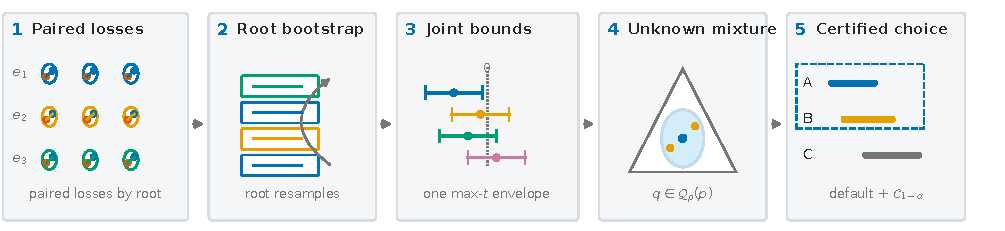
\includegraphics[width=\linewidth]{figures/method.pdf}
  \caption{HRMS consumes a frozen validation loss table: paired losses are
  resampled at the independent root, enclosed jointly, and propagated through
  mixture uncertainty to an operational default and a robust-optimal
  non-exclusion set. Training precedes, and target evaluation follows, this
  pipeline.}
  \label{fig:method}
\end{figure}

\section{Closest related work and problem setup}
\label{sec:setup}

\paragraph{Closest work.}
MRO minimizes worst-case excess risk rather than worst-case absolute risk and can avoid selecting a model merely because an environment has high irreducible risk \citep{agarwal2022mro}.  HRMS adopts this regret principle; unlike that learning-theoretic treatment, we select from a frozen finite library and place simultaneous uncertainty on its environment-wise pairwise losses under clustered sampling.  Model confidence sets retain statistically indistinguishable forecasting models \citep{hansen2011mcs}; comparisons with the best and bootstrap reality checks likewise address multiplicity after searching many specifications \citep{hsu1981best,white2000reality}.  Online conformal model prediction sets target the next-period best model under nonstationary time series \citep{li2026online}; HRMS instead targets an offline robust-mixture optimum from clustered data.

MANDOLINE estimates target performance using labeled source data, an unlabeled target sample, and user-specified shift slices \citep{chen2021mandoline}; HRMS addresses the no-target-data case.  Pairwise model assessment has also been studied under temporal shift \citep{han2024model}.  Recent model routing handles unknown source-domain mixtures by learning an input-dependent router \citep{dann2025routing}; HRMS makes one pre-deployment library choice and quantifies finite validation uncertainty.  Cluster bootstrap, studentized bootstrap intervals, and bootstrap multiple-comparison procedures are established tools \citep{field2007cluster,hall1988bootstrap,westfall2011bootstrap}, and $\phi$-divergence ambiguity sets are standard in robust optimization \citep{bental2013phi}.  We do not claim these components separately.

\paragraph{Frozen library and independent splits.}
Let $\M=\{1,\ldots,M\}$ be candidate configurations fixed before inspecting selection rankings.  Records are split into $D_{\rm train}$, $D_{\rm select}$, and $D_{\rm test}$ at the highest independent root-cluster level.  All architecture, representation, hyperparameter, seed, checkpoint, training-data, calibration, and prediction-file identifiers are registered before selection.  Models and probability calibrators use training data only.  HRMS receives only frozen $D_{\rm select}$ predictions; $D_{\rm test}$ losses are excluded from selection and used only by the evaluator.  This governance is part of the estimand: simultaneous inference cannot cover candidates invented after observing selection outcomes.

For selection record $i$, let $e_i\in[E]$ be its environment, $c_i$ its independent root cluster, $y_i\in\{0,1\}$ its label, $p_{im}$ candidate $m$'s probability, and $w_i>0$ a prespecified sampling weight.  We use bounded Brier loss
$\ell_{im}=(p_{im}-y_i)^2\in[0,1]$; AUROC, AUPRC, calibration error, and balanced accuracy are descriptive only.

\paragraph{Two risk estimands.}
Let $I_{C,e}$ denote the nonempty records contributed to environment $e$ by a randomly sampled root $C$, and define $A_{C,m,e}=\sum_{i\in I_{C,e}}w_i\ell_{im}$ and $W_{C,e}=\sum_{i\in I_{C,e}}w_i$.  The two population targets are
\begin{equation}
R^{\rm obs}_{m,e}=\frac{\mathbb E[A_{C,m,e}]}{\mathbb E[W_{C,e}]},
\qquad
R^{\rm cl}_{m,e}=\mathbb E\!\left[\frac{A_{C,m,e}}{W_{C,e}}\right].
\label{eq:estimands}
\end{equation}
The first samples records proportionally to their prespecified weights; the second gives every represented root equal total weight.  Their sample estimators are, respectively,
\begin{equation}
\widehat R^{\rm obs}_{m,e}=
\frac{\sum_{i:e_i=e}w_i\ell_{im}}{\sum_{i:e_i=e}w_i}.
\label{eq:obsrisk}
\end{equation}
The cluster-balanced estimator first averages within each of the $C_e$ roots represented in environment $e$,
\begin{equation}
\widehat R^{\rm cl}_{m,e}=\frac{1}{C_e}\sum_{c:I_{ce}\ne\varnothing}
\frac{\sum_{i\in I_{ce}}w_i\ell_{im}}{\sum_{i\in I_{ce}}w_i},
\qquad I_{ce}=\{i:c_i=c,e_i=e\}.
\label{eq:clrisk}
\end{equation}
The former permits large roots to contribute more; the latter targets a random root.  Neither is universally preferable, so disagreement is reported rather than hidden.  We choose one estimand before selection and write it as $R_{m,e}$ below.

\paragraph{Target mixtures and pairwise differences.}
The unknown target is $q\in\Delta^E$, a mixture of the represented environment distributions.  Define
\begin{equation}
\begin{aligned}
\Delta_{mk,e}&=R_{m,e}-R_{k,e}, &
R_m(q)&=\sum_e q_eR_{m,e},\\
G_m(q)&=R_m(q)-\min_kR_k(q), &
G_m(q)&=\max_k\sum_eq_e\Delta_{mk,e}.
\end{aligned}
\label{eq:regret}
\end{equation}
Because candidates share validation records, inference targets $\ell_{im}-\ell_{ik}$, not two independently estimated risks.

\section{Hierarchical Robust Model Selection}
\label{sec:method}

\subsection{Paired delete-root bootstrap-t and simultaneous bounds}

Let $\widehat\Delta_{mk,e}=\widehat R_{m,e}-\widehat R_{k,e}$ for either estimand above.  If roots are nested within environments, each environment is a resampling block with $C_g=C_e$ roots.  If any root spans environments, all $C_g=C$ roots and all environments form one global block: deletion and resampling act jointly on every record of a spanning root.  Named lower levels are not separately resampled, and every operation is shared across candidates.

For root $c$ in block $g$, delete it and recompute $\widehat R^{(-c)}_{m,e}$ for each environment $e$ in that block.  Define risk pseudovalues $Z_{c,m,e}=C_g\widehat R_{m,e}-(C_g-1)\widehat R^{(-c)}_{m,e}$ and paired pseudocontrasts $P_{c,mk,e}=Z_{c,m,e}-Z_{c,k,e}$.  Let $\bar P_{mk,e}$ and $\widehat s_{mk,e}=\operatorname{sd}_c(P_{c,mk,e})/\sqrt{C_g}$ be their block mean and jackknife standard error.  After centering $X_{c,mk,e}=P_{c,mk,e}-\bar P_{mk,e}$, replicate $b$ resamples $C_g$ root rows within each block and computes their mean $\bar X^{*(b)}_{mk,e}$ and standard error $\widehat s^{*(b)}_{mk,e}$.  Over $\mathcal A=\{(m,k,e):m<k,\widehat s_{mk,e}>0\}$, the joint statistic is
\begin{equation}
T_b=\max_{(m,k,e)\in\mathcal A}
\left|\frac{\bar X^{*(b)}_{mk,e}}{\widehat s^{*(b)}_{mk,e}}\right|,
\qquad c_{1-\alpha}=\operatorname{quantile}^{\rm higher}_{1-\alpha}\{T_b\}_{b=1}^B.
\label{eq:maxt}
\end{equation}
For loss range $[a,b]$, the bounds are centered at the original risk contrast and clipped to its attainable range:
\begin{equation}
L_{mk,e}=\max\{a-b,\widehat\Delta_{mk,e}-c_{1-\alpha}\widehat s_{mk,e}\},\quad
U_{mk,e}=\min\{b-a,\widehat\Delta_{mk,e}+c_{1-\alpha}\widehat s_{mk,e}\}.
\label{eq:bounds}
\end{equation}
For Brier loss this range is $[-1,1]$.  We compute only $m<k$, impose exact antisymmetry, and set the diagonal to zero.  A zero interval is permitted only for a structural duplicate declared before selection and passing exact observation-wise loss-vector equality; observed equality never marks a pair automatically, and the guarantee assumes the declaration is substantively correct.  A nonstructural coordinate with zero jackknife scale receives the full attainable interval and triggers a diagnostic.  Raw root-cluster bootstrap-t (\texttt{raw\_bootstrap\_t}) and ordinary fixed-denominator bootstrap max-t (\texttt{fixed\_max\_t}) are prespecified ablations, not the \texttt{jackknife\_bootstrap\_t} default.  The result object records the exact choice in \texttt{calibration\_method}.  The intended event is
\begin{equation}
\mathcal J=\{L_{mk,e}\leq\Delta_{mk,e}\leq U_{mk,e}
\ \text{for all }m,k,e\},\qquad \Pr(\mathcal J)\approx1-\alpha.
\label{eq:joint}
\end{equation}
This approximation, not finite-sample exactness, is what the simulations test.  We use $\alpha=.05$, $B=999$ for headline simulations and $B=1{,}999$ for the real-data analysis.

\subsection{Ambiguous mixtures and robust regret certificates}

Let $p$ lie in the interior of $\Delta^E$---that is, $p_e>0$ for every $e$---and be a prespecified nominal mixture, uniform by default.  For radius $\rho\geq0$, use the chi-squared ambiguity set
\begin{equation}
\Q_\rho(p)=\left\{q\in\Delta^E:
\sum_{e=1}^E\frac{(q_e-p_e)^2}{p_e}\leq\rho\right\}.
\label{eq:ambiguity}
\end{equation}
At $\rho=0$ this is $\{p\}$; when $\rho\geq\max_e(1/p_e-1)$ it contains the full simplex.  We never tune $\rho$ with test labels.  For uniform $p$, the largest permitted weight on one environment is $\min\{1,[1+\sqrt{\rho(E-1)}]/E\}$; we report this scale alongside $\rho$.

The true robust regret and its data-dependent sandwich are
\begin{align}
\Gamma_m(\rho)&=\max_{q\in\Q_\rho(p)}\max_{k\in\M}\sum_eq_e\Delta_{mk,e},\label{eq:truegamma}\\
\RRlo_m(\rho)&=\max_{q\in\Q_\rho(p)}\max_{k\in\M}\sum_eq_eL_{mk,e},\qquad
\RRhi_m(\rho)=\max_{q\in\Q_\rho(p)}\max_{k\in\M}\sum_eq_eU_{mk,e}.
\label{eq:gammabounds}
\end{align}
Including $k=m$ ensures all three are nonnegative.  Because $\M$ is finite, each quantity is the maximum over $k$ of a small convex optimization in $E$ variables.  The implementation uses a specialized analytic active-set solver in NumPy and checks it against independent SciPy/SLSQP and CVXPY reference formulations in unit tests.  Full-simplex ambiguity reduces each inner problem to $\max_e U_{mk,e}$ (or its $L$ and $\Delta$ analogues).

The default decision and robust model confidence set are
\begin{equation}
\widehat m\in\argmin_m\RRhi_m(\rho),\qquad
\mathcal C_{1-\alpha}(\rho)=
\left\{m:\RRlo_m(\rho)\leq\min_j\RRhi_j(\rho)\right\}.
\label{eq:decision}
\end{equation}
Numerical upper-certificate ties (tolerance $10^{-12}$, ignored in the formal argmin) are broken by point-estimated robust regret, then canonical model identifier.  HRMS reports $\widehat m$, its certificate, $\mathcal C_{1-\alpha}$, cluster counts, a $\rho$ path, and the calibration method.  It also reports the raw root-bootstrap frequency with which each candidate minimizes point-estimated robust regret; this auxiliary diagnostic does not refit the HRMS envelope and is not a posterior probability.
Because $L\leq U$, $\RRlo_m\leq\RRhi_m$ for every $m$, so the selected candidate belongs to the returned set by construction.  Candidates outside the set are ruled out as robust-optimal only to the extent that the joint envelope is calibrated.

\section{Conditional guarantees}
\label{sec:theory}

The guarantee separates a deterministic propagation result from the statistical calibration of $\mathcal J$.

\begin{theorem}[Simultaneous robust-regret sandwich]
\label{thm:sandwich}
For any nonempty $\Q\subseteq\Delta^E$, define the three functionals in \eqref{eq:truegamma}--\eqref{eq:gammabounds} with $\Q$ replacing $\Q_\rho(p)$.  On the event $\mathcal J$, simultaneously for every $m\in\M$,
$\RRlo_m(\Q)\leq\Gamma_m(\Q)\leq\RRhi_m(\Q)$.
\end{theorem}
\begin{proof}
For fixed $(m,k,q)$, nonnegativity of $q_e$ and the componentwise bounds give
$\sum_eq_eL_{mk,e}\leq\sum_eq_e\Delta_{mk,e}\leq\sum_eq_eU_{mk,e}$.
Maximizing each term over the same $(k,q)$ preserves both inequalities.  Because $\mathcal J$ holds for all pairs and environments, the conclusion holds for all $m$ simultaneously.
\end{proof}

\begin{corollary}[Coverage of the robust model confidence set]
\label{cor:mcs}
On $\mathcal J$, every $m^\star\in\argmin_m\Gamma_m(\rho)$ belongs to $\mathcal C_{1-\alpha}(\rho)$.  Consequently, $\Pr\{\argmin_m\Gamma_m(\rho)\subseteq\mathcal C_{1-\alpha}(\rho)\}\geq\Pr(\mathcal J)$.
\end{corollary}
\begin{proof}
$\RRlo_{m^\star}\leq\Gamma_{m^\star}=\min_j\Gamma_j\leq\min_j\RRhi_j$ on $\mathcal J$, which is exactly the membership rule in \eqref{eq:decision}.
\end{proof}

\begin{corollary}[Oracle slack]
\label{prop:oracle}
On $\mathcal J$, define the one-sided envelope slack
$\eta=\max_{m,k,e}\{U_{mk,e}-\Delta_{mk,e}\}$.  For any robust optimum $m^\star$,
\begin{equation}
\Gamma_{\widehat m}(\rho)\leq\Gamma_{m^\star}(\rho)+\eta.
\label{eq:oracle}
\end{equation}
In particular, if every symmetric interval has half-width at most $\epsilon$, then $\eta\leq2\epsilon$ and the valid generic bound is $\Gamma_{\widehat m}\leq\Gamma_{m^\star}+2\epsilon$.
\end{corollary}
\begin{proof}
For any $m$, simplex weights imply $\RRhi_m\leq\Gamma_m+\eta$.  Thus
$\Gamma_{\widehat m}\leq\RRhi_{\widehat m}\leq\RRhi_{m^\star}
\leq\Gamma_{m^\star}+\eta$.  If an interval is $[\widehat\Delta-\epsilon,\widehat\Delta+\epsilon]$ and contains $\Delta$, its upper endpoint can exceed $\Delta$ by $2\epsilon$; a one-$\epsilon$ statement would require directly assuming $U-\Delta\leq\epsilon$.
\end{proof}

These results are conditional: they do not prove exact finite-sample bootstrap coverage.  Root clusters must be independent (or satisfy an appropriate weak-dependence regime), every environment needs enough roots, and the risk estimators must be regular.  The familiar equal-cluster design effect $1+(s-1)\tau$ gives $N_{\rm eff}\approx N/[1+(s-1)\tau]$ for size $s$ and intracluster correlation $\tau$, illustrating why locus-level IID uncertainty can be badly optimistic.  HRMS warns rather than extrapolates when root counts are small.

\section{Evaluation design}
\label{sec:experiments}

We freeze every configuration before its final run and report completed results only from content-addressed outputs.  Calibration baselines are observation-level IID marginal and Bonferroni intervals, cluster-aware marginal intervals, a fixed-denominator paired max-$t$ bootstrap, and a raw paired cluster bootstrap-$t$.  Selection baselines are the uniform nominal environment mean, worst environment, point-estimate robust risk, point-estimate robust regret, and HRMS at $\rho=0$.  Population risks in simulation and held-out application losses are excluded from selection and used only for evaluation.

\begin{table}[t]
\centering
\caption{Evaluation settings.  TE counts are totals; CivilComments observations and article roots are validation/test.}
\label{tab:data}
\scriptsize
\setlength{\tabcolsep}{3pt}
\begin{tabular}{lccccc}
\toprule
Task & Envs. & Obs. & Roots & Candidates & Target mixtures \\
\midrule
Calibration simulation & 3 & synthetic & 25/env. & 10 & known \\
Rank-reversal simulation & 8 & synthetic & 25/env. & 8 & $\Q_{1}$ \\
Public TE--cCRE & 4 & 22,590 & 10,920 & 24 & TE families \\
CivilComments-derived & 8 & \CivilObservations & \CivilRoots & \CivilCandidates & identities \\
\bottomrule
\end{tabular}
\end{table}

\subsection{Controlled simulations}

\paragraph{A: interval calibration.}
We generate bounded correlated candidate losses
\begin{equation}
L_{cjem}=\operatorname{logit}^{-1}(\mu_{m,e}+a_{c,e}+b_{c,m}+\varepsilon_{cjem}),
\label{eq:simloss}
\end{equation}
where $c$ is a root, $j$ an observation, $e$ an environment, and $m$ a candidate.  Shared difficulty $a_{c,e}$ and candidate--cluster interaction $b_{c,m}$ induce both intracluster dependence and paired candidate correlation; Gauss--Hermite quadrature gives the population risks.  The headline setting has three environments, ten candidates, 25 roots per environment, mean root size ten, moderate size imbalance, candidate correlation $.7$, and latent-Gaussian ICC $\{0,.1,.3,.5\}$; the ICC of the bounded transformed losses is not numerically identical.  Sensitivities use 10--100 roots, 20 candidates, eight environments, equal or severe size imbalance, and candidate correlations $.2$ and $.95$.  Primary outcomes are joint interval coverage, width, and family-wise error.

\paragraph{B: rank reversal.}
With $Y\sim\operatorname{Bernoulli}(.5)$, we draw
\begin{equation}
X_{\rm stable}=(2Y-1)\mu+u_c+\epsilon,\qquad
X_{\rm spur}=(2Y-1)\gamma_e+v_c+\zeta,
\label{eq:ranksim}
\end{equation}
and change the sign and magnitude of $\gamma_e$ across environments.  Candidate predictors use prespecified weights on stable and spurious features, regularization, and temperature.  We measure target regret, oracle-selection frequency, false-singleton rate, and confidence-set coverage and size against a seed-fixed 500,000-draw reference population.  The headline design, frozen before its run, uses 500 Monte Carlo repetitions and $B=999$.  Hypotheses are directional but not guaranteed: IID and marginal intervals should degrade with ICC and library size; pairing should narrow bounds when loss correlation is positive; robustness should help under rank reversal but can be conservative without rank reversal.

\begin{figure}[t]
  \centering
  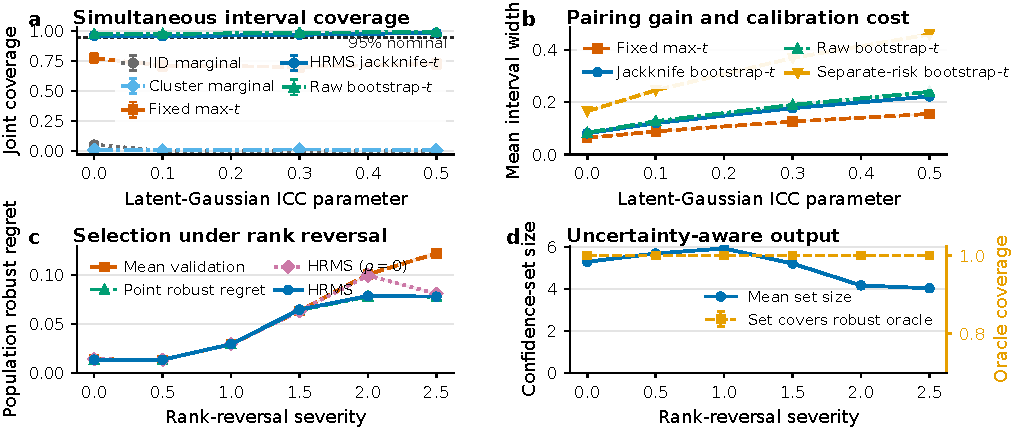
\includegraphics[width=\linewidth]{figures/simulation.pdf}
  \caption{Simulations, 500 Monte Carlo repetitions and $B=999$.  (a--b) Joint coverage and mean width of simultaneous intervals versus the latent-Gaussian ICC parameter; error bars are $\pm1.96$ Monte Carlo standard errors (coverage bars clipped to $[0,1]$).  ``Raw paired'' applies bootstrap-$t$ directly to root resamples; ``cluster marginal'' has no multiplicity correction; ``separate risk'' derives contrasts from simultaneous absolute-risk intervals and discards paired covariance.  (c) Reference-population robust regret at $\rho=1$ as one represented environment increasingly reverses its spurious signal; bands are $\pm1.96$ Monte Carlo standard errors.  (d) HRMS confidence-set size and robust-oracle coverage.}
  \label{fig:simulation}
\end{figure}

\paragraph{Results.}
The default jackknife bootstrap-$t$ attains $.958$--$.986$ joint coverage over ICC $0$--$.5$ (Figure~\ref{fig:simulation}a).  Simultaneous separate-risk intervals cover $1.000$ throughout but are conservative: exploiting pairing makes HRMS intervals 51.0--52.0\% narrower.  Raw paired bootstrap-$t$ is also slightly conservative ($.974$--$.996$), whereas the fixed-denominator max-$t$ covers only $.702$--$.776$.  Marginal cluster intervals cover at most $.012$ jointly, illustrating that dependence-aware standard errors alone do not address selection across 135 pair--environment coordinates (their coordinate coverage is $.921$--$.931$).  IID Bonferroni coverage falls from $.966$ at ICC zero to zero at ICC $.5$.  At ICC $.3$, mean widths are $.177$ for HRMS, $.369$ for separate-risk, and $.126$ for the under-covering fixed max-$t$.

In the rank-reversal study, the 500,000-draw reference robust optimum changes as one of eight represented environments reverses its spurious signal (Figure~\ref{fig:simulation}c).  At the strongest severity, HRMS selects that optimum in all 500 repetitions and has reference regret $.07783$, versus $.12203$ for uniform-environment mean selection, a 36.2\% reduction (paired difference $-.04420$, 95\% Monte Carlo $t_{499}$ interval $[-.04641,-.04200]$).  Point-estimate robust-regret selection also reaches $.07783$: HRMS does not improve its point decision in this high-separation regime.  Its added output is conservative and set-valued: the robust optimum is covered in every repetition at every severity, no false singleton occurs, and mean set size is $5.29$ at severity zero, peaks at $5.92$, and is $4.02$ at the strongest reversal.  HRMS is not uniformly best: at severity $1.5$ its regret exceeds the nominal mean by $.00144$ on average (95\% interval $[.00106,.00183]$).

\subsection{Public TE-associated cCRE benchmark}

Our primary clustered application predicts association between an hg38 TE copy and an enhancer-like ENCODE candidate cis-regulatory element (cCRE), not causality.  We intersect SCREEN Registry V4 pELS/dELS \citep{moore2026registry} with UCSC Repeat Browser 2020 loci \citep{fernandes2020repeatbrowser}.  Following \citet{du2024regulatory}, a positive TE overlaps at least 50\% of one pELS/dELS cCRE; a strict control's TE interval expanded by 250 bp overlaps no Registry V4 cCRE.  Controls are matched without replacement within exact RepeatMasker subfamily and chromosome on full oriented TE-copy GC (caliper $.03$) and relative length (caliper $.20$), then receive the positive's strand-aware normalized window position.  The frozen cohort has one positive and one matched control per pair, capped at 500 pairs per exact subfamily, so risks and calibration target this balanced benchmark rather than natural cCRE prevalence or subfamily composition.  A pre-training amendment clarified full-TE GC matching because control windows exist only after anchor transfer.  Test positive-minus-negative mean window-GC residuals are $.00939/.00705/.00663/.01590$ for ERVL/L1/L2/MIR; we also report a GC/length diagnostic.

The operational root is the transitive union of matched-pair edges and global MMseqs2 \citep{steinegger2017mmseqs2} 80\%-identity/80\%-bidirectional-coverage components on full TE copies and 512-bp windows.  Performance-blind gates removed Alu in the pilot (largest root 80.4\%) and ERV1, ERVL-MaLR, and hAT-Charlie in production (8.53\%, 18.6\%, 5.23\%); the frozen select/test rule required every held-out root below 5\%.  ERVL, L1, L2, and MIR passed (maximum 4.22\%).  The 22,590 loci/10,920 roots split train/select/test as 13,702/4,450/4,438 loci and 6,552/2,184/2,184 roots, without an 80/80 cross-split edge.  The 24 frozen CPU TF--IDF candidates combine four sequence views with logistic regression, averaged-SGD logistic regression, and complement Naive Bayes; diagnostics are not candidates.

With observation weighting, $B=1{,}999$, $\alpha=.05$, and $\rho=.25$, HRMS's operational default is 128-bp $k=6$ logistic regression with $C=.1$ (C03), with upper certificate $.012609$ and the same choice at every reported radius on the prespecified path.  A separate 500-replicate raw-root diagnostic gives $.894$ point-selection stability.  Yet the set is $24/24$ at $\rho=.25$, $23$ at $\rho=1$, and $22$ on the full simplex, so no winner is identified.  All five primary selectors choose C03 and therefore coincide over 576 fixed mixtures within $\rho\leq.25$ (Figure~\ref{fig:te}b); this is not a regret-dominance result.

The test-loss table was not inspected by selection; the evaluator first read and aggregated it after persisting and hashing the selection bundle.  On that held-out table, C03's plug-in robust regret is $.001383$, versus $.000963$ for the plug-in oracle C04 (the same model with $C=1$); C03's selection-data regret interval contains its held-out plug-in reference, and the set contains C04 and every test optimum.  Pairwise environment-rank Kendall correlations span $.232$--$.906$; winners are 128-bp averaged SGD for ERVL, C04 for L1, 256-bp $k=6$ logistic $C=1$ for L2, and its 512-bp $C=.1$ analogue for MIR (Figure~\ref{fig:te}a).  C03's macro test Brier/AUROC/AUPRC/ECE/balanced accuracy are $.224433/.689741/.664835/.042602/.628820$; the GC/length diagnostic's Brier/AUROC/AUPRC are $.248161/.549317/.543929$.

\begin{figure}[t]
  \centering
  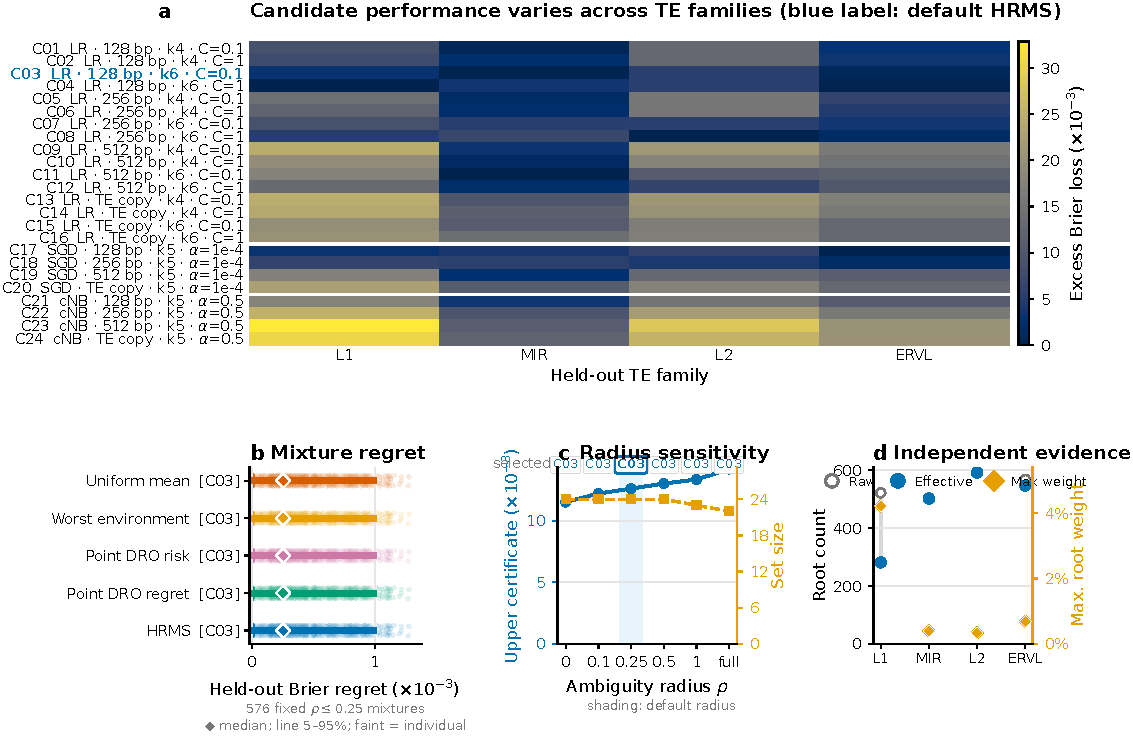
\includegraphics[width=\linewidth]{figures/te_public.pdf}
  \caption{Held-out public TE--cCRE evaluation after selection was persisted.  (a) Test excess Brier risk reveals family-specific rank reversals; blue marks C03.  (b) The five primary selectors coincide over 576 fixed mixtures within $\rho\leq.25$.  (c) C03 is selected throughout the radius path, while the 95\% set remains large.  (d) Selection raw/effective roots are 567/546 (ERVL), 521/281 (L1), 593/591 (L2), and 503/501 (MIR); the largest held-out root weight is 4.22\%.}
  \label{fig:te}
\end{figure}

\subsection{Derived CivilComments task and root sensitivity}

CivilComments is a WILDS toxicity dataset \citep{koh2021wilds,borkan2019civilcomments}.  We retain comments with exactly one of eight identity scores $\geq.5$ (male, female, LGBTQ, Christian, Muslim, other religion, Black, White) and binarize toxicity at $.5$, yielding a derived mixture task rather than the leaderboard setting.  The content-addressed CC0-1.0 source feeds 12 frozen TF--IDF logistic configurations: word uni/uni-bigrams and character-boundary 3--5/4--6-grams, each with $C\in\{.1,1,10\}$.  Training-only Platt calibration precedes selection on 12,823 comments/3,046 article roots; held-out test, evaluated after selection was frozen, has 37,226/8,792.

Article ID is the highest available dependence unit; spanning roots are resampled globally, with $B=1{,}999$, $\alpha=.05$, and $\rho=.25$.  Minimum pairwise test-environment Kendall $\tau$ is $.394$.  HRMS's operational default is word-unigram $C=1$, but its 95\% set retains all 12 and contains the plug-in test optimum; no candidate exceeds $.406$ raw-bootstrap point stability.  In a post-test, intentionally misspecified IID-comment sensitivity, the point winner changes to character 4--6-gram $C=1$, yet both sets remain $12/12$.  Table~\ref{tab:civil} shows that this, too, is not regret dominance.

\begin{table}[t]
\centering
\scriptsize
\caption{Derived CivilComments at $\rho=.25$ on one held-out test table evaluated after selection was frozen; the full HRMS set contains the test optimum.}
\label{tab:civil}
\setlength{\tabcolsep}{3pt}
\begin{tabular}{lcccccc}
\toprule
 & Uniform & Worst env. & Point risk & Point regret & HRMS ($\rho=0$) & Full HRMS \\
\midrule
Test regret & $.000277$ & $.001562$ & $.000277$ & $.0000391$ & $.0000391$ & $.001562$ \\
Set size & -- & -- & -- & -- & -- & $12$ \\
\bottomrule
\end{tabular}
\end{table}

\section{Limitations, broader impact, and conclusion}
\label{sec:limitations}

HRMS guarantees only prevalence mixtures of represented environments with within-environment risks fixed, not conditional shift.  The library and radius must be fixed without inspecting test outcomes; bootstrap calibration is approximate and weak with few roots.  Homology components and article IDs are root proxies, so residual dependence may remain.  Radius and weighting are modeling choices, and the outer set can be conservative or vacuous---as both applications show---and does not optimize size.  HRMS cannot repair leakage or a poor library.  TE cCRE labels are noncausal, controls may have unmeasured activity, and residual window-GC imbalance remains.  Both real libraries are lightweight TF--IDF variants, so point utility for deep or foundation-model libraries is untested.  The full TE set is non-identification, not equivalence.

Runs were CPU-only (Intel i5-13420H, 8 cores/12 threads, 30~GiB RAM).  Approximate wall times for simulation coverage/decision and CivilComments were 4,170/486/272~s (simulation peak RSS 233/349~MiB).  Failed/final TE graph runs took 9~h 23~min/33~min; vectorization plus fitting took about 82~s and evaluation 67~s.  CivilComments peak memory and total development overhead were not recorded.

Certificates establish neither safety, fairness, nor domain validity; identity mentions are attributes, not people, and no comments are redistributed.  Simulations are near nominal and robustness can beat nominal averaging, but both applications return full sets.  HRMS qualifies selection uncertainty rather than promising gains.

\clearpage
\bibliographystyle{plainnat}
\bibliography{references}

\section*{NeurIPS Paper Checklist}

\begin{enumerate}

\item {\bf Claims}
    \item[] Question: Do the main claims made in the abstract and introduction accurately reflect the paper's contributions and scope?
    \item[] Answer: \answerYes{}
    \item[] Justification: The abstract and Sections~\ref{sec:intro}, \ref{sec:experiments}, and \ref{sec:limitations} state the fixed-library and represented-mixture scope, distinguish the conditional theorem from empirical bootstrap calibration, and limit empirical claims to the reported simulations, public TE--cCRE benchmark, and derived CivilComments task.
    \item[] Guidelines:
    \begin{itemize}
        \item The answer \answerNA{} means that the abstract and introduction do not include the claims made in the paper.
        \item The abstract and/or introduction should clearly state the claims made, including the contributions made in the paper and important assumptions and limitations. A \answerNo{} or \answerNA{} answer to this question will not be perceived well by the reviewers. 
        \item The claims made should match theoretical and experimental results, and reflect how much the results can be expected to generalize to other settings. 
        \item It is fine to include aspirational goals as motivation as long as it is clear that these goals are not attained by the paper. 
    \end{itemize}

\item {\bf Limitations}
    \item[] Question: Does the paper discuss the limitations of the work performed by the authors?
    \item[] Answer: \answerYes{}
    \item[] Justification: Section~\ref{sec:limitations} discusses the represented-environment assumption, fixed library and radius, few-root behavior, bootstrap approximation, estimand choice, residual article dependence, TE label and window-composition limitations, computational scaling, and fairness and safety limits.
    \item[] Guidelines:
    \begin{itemize}
        \item The answer \answerNA{} means that the paper has no limitation while the answer \answerNo{} means that the paper has limitations, but those are not discussed in the paper. 
        \item The authors are encouraged to create a separate ``Limitations'' section in their paper.
        \item The paper should point out any strong assumptions and how robust the results are to violations of these assumptions (e.g., independence assumptions, noiseless settings, model well-specification, asymptotic approximations only holding locally). The authors should reflect on how these assumptions might be violated in practice and what the implications would be.
        \item The authors should reflect on the scope of the claims made, e.g., if the approach was only tested on a few datasets or with a few runs. In general, empirical results often depend on implicit assumptions, which should be articulated.
        \item The authors should reflect on the factors that influence the performance of the approach. For example, a facial recognition algorithm may perform poorly when image resolution is low or images are taken in low lighting. Or a speech-to-text system might not be used reliably to provide closed captions for online lectures because it fails to handle technical jargon.
        \item The authors should discuss the computational efficiency of the proposed algorithms and how they scale with dataset size.
        \item If applicable, the authors should discuss possible limitations of their approach to address problems of privacy and fairness.
        \item While the authors might fear that complete honesty about limitations might be used by reviewers as grounds for rejection, a worse outcome might be that reviewers discover limitations that aren't acknowledged in the paper. The authors should use their best judgment and recognize that individual actions in favor of transparency play an important role in developing norms that preserve the integrity of the community. Reviewers will be specifically instructed to not penalize honesty concerning limitations.
    \end{itemize}

\item {\bf Theory assumptions and proofs}
    \item[] Question: For each theoretical result, does the paper provide the full set of assumptions and a complete (and correct) proof?
    \item[] Answer: \answerYes{}
    \item[] Justification: Section~\ref{sec:theory} states the joint-coverage and ambiguity-set conditions, numbers and cross-references each result, gives complete proofs, and explicitly separates deterministic propagation from bootstrap calibration.
    \item[] Guidelines:
    \begin{itemize}
        \item The answer \answerNA{} means that the paper does not include theoretical results. 
        \item All the theorems, formulas, and proofs in the paper should be numbered and cross-referenced.
        \item All assumptions should be clearly stated or referenced in the statement of any theorems.
        \item The proofs can either appear in the main paper or the supplemental material, but if they appear in the supplemental material, the authors are encouraged to provide a short proof sketch to provide intuition. 
        \item Inversely, any informal proof provided in the core of the paper should be complemented by formal proofs provided in appendix or supplemental material.
        \item Theorems and Lemmas that the proof relies upon should be properly referenced. 
    \end{itemize}

    \item {\bf Experimental result reproducibility}
    \item[] Question: Does the paper fully disclose all the information needed to reproduce the main experimental results of the paper to the extent that it affects the main claims and/or conclusions of the paper (regardless of whether the code and data are provided or not)?
    \item[] Answer: \answerNo{}
    \item[] Justification: The paper gives the algorithms, generators, frozen headline dimensions, public TE construction and performance-blind gates, and evaluation protocols, and a complete content-addressed reproducibility artifact has been prepared locally; however, that artifact has not yet been made available through an anonymous submission URL.
    \item[] Guidelines:
    \begin{itemize}
        \item The answer \answerNA{} means that the paper does not include experiments.
        \item If the paper includes experiments, a \answerNo{} answer to this question will not be perceived well by the reviewers: Making the paper reproducible is important, regardless of whether the code and data are provided or not.
        \item If the contribution is a dataset and\slash or model, the authors should describe the steps taken to make their results reproducible or verifiable. 
        \item Depending on the contribution, reproducibility can be accomplished in various ways. For example, if the contribution is a novel architecture, describing the architecture fully might suffice, or if the contribution is a specific model and empirical evaluation, it may be necessary to either make it possible for others to replicate the model with the same dataset, or provide access to the model. In general. releasing code and data is often one good way to accomplish this, but reproducibility can also be provided via detailed instructions for how to replicate the results, access to a hosted model (e.g., in the case of a large language model), releasing of a model checkpoint, or other means that are appropriate to the research performed.
        \item While NeurIPS does not require releasing code, the conference does require all submissions to provide some reasonable avenue for reproducibility, which may depend on the nature of the contribution. For example
        \begin{enumerate}
            \item If the contribution is primarily a new algorithm, the paper should make it clear how to reproduce that algorithm.
            \item If the contribution is primarily a new model architecture, the paper should describe the architecture clearly and fully.
            \item If the contribution is a new model (e.g., a large language model), then there should either be a way to access this model for reproducing the results or a way to reproduce the model (e.g., with an open-source dataset or instructions for how to construct the dataset).
            \item We recognize that reproducibility may be tricky in some cases, in which case authors are welcome to describe the particular way they provide for reproducibility. In the case of closed-source models, it may be that access to the model is limited in some way (e.g., to registered users), but it should be possible for other researchers to have some path to reproducing or verifying the results.
        \end{enumerate}
    \end{itemize}


\item {\bf Open access to data and code}
    \item[] Question: Does the paper provide open access to the data and code, with sufficient instructions to faithfully reproduce the main experimental results, as described in supplemental material?
    \item[] Answer: \answerNo{}
    \item[] Justification: The implementation and content-addressed result bundle are prepared, but no anonymous public archive or supplemental code bundle is yet cited.  CivilComments is independently available under CC0-1.0, SCREEN and Repeat Browser are public sources, and source records rather than redistributed comment text are used.
    \item[] Guidelines:
    \begin{itemize}
        \item The answer \answerNA{} means that paper does not include experiments requiring code.
        \item Please see the NeurIPS code and data submission guidelines (\url{https://neurips.cc/public/guides/CodeSubmissionPolicy}) for more details.
        \item While we encourage the release of code and data, we understand that this might not be possible, so \answerNo{} is an acceptable answer. Papers cannot be rejected simply for not including code, unless this is central to the contribution (e.g., for a new open-source benchmark).
        \item The instructions should contain the exact command and environment needed to run to reproduce the results. See the NeurIPS code and data submission guidelines (\url{https://neurips.cc/public/guides/CodeSubmissionPolicy}) for more details.
        \item The authors should provide instructions on data access and preparation, including how to access the raw data, preprocessed data, intermediate data, and generated data, etc.
        \item The authors should provide scripts to reproduce all experimental results for the new proposed method and baselines. If only a subset of experiments are reproducible, they should state which ones are omitted from the script and why.
        \item At submission time, to preserve anonymity, the authors should release anonymized versions (if applicable).
        \item Providing as much information as possible in supplemental material (appended to the paper) is recommended, but including URLs to data and code is permitted.
    \end{itemize}


\item {\bf Experimental setting/details}
    \item[] Question: Does the paper specify all the training and test details (e.g., data splits, hyperparameters, how they were chosen, type of optimizer) necessary to understand the results?
    \item[] Answer: \answerYes{}
    \item[] Justification: Sections~\ref{sec:experiments} and its task subsections specify the generators, repetitions, bootstrap counts, library sizes, training/calibration separation, TE matching and homology gates, ambiguity radii, resampling units, losses, and evaluation metrics needed to interpret the results.
    \item[] Guidelines:
    \begin{itemize}
        \item The answer \answerNA{} means that the paper does not include experiments.
        \item The experimental setting should be presented in the core of the paper to a level of detail that is necessary to appreciate the results and make sense of them.
        \item The full details can be provided either with the code, in appendix, or as supplemental material.
    \end{itemize}

\item {\bf Experiment statistical significance}
    \item[] Question: Does the paper report error bars suitably and correctly defined or other appropriate information about the statistical significance of the experiments?
    \item[] Answer: \answerYes{}
    \item[] Justification: Figure~\ref{fig:simulation} reports $\pm1.96$ Monte Carlo standard errors over 500 independently generated datasets, and the main paired regret contrast uses a $t_{499}$ interval.  TE and CivilComments are explicitly reported as single held-out-table evaluations performed after selections were frozen; TE mixture points summarize 576 fixed mixtures rather than repeated-sample uncertainty.
    \item[] Guidelines:
    \begin{itemize}
        \item The answer \answerNA{} means that the paper does not include experiments.
        \item The authors should answer \answerYes{} if the results are accompanied by error bars, confidence intervals, or statistical significance tests, at least for the experiments that support the main claims of the paper.
        \item The factors of variability that the error bars are capturing should be clearly stated (for example, train/test split, initialization, random drawing of some parameter, or overall run with given experimental conditions).
        \item The method for calculating the error bars should be explained (closed form formula, call to a library function, bootstrap, etc.)
        \item The assumptions made should be given (e.g., Normally distributed errors).
        \item It should be clear whether the error bar is the standard deviation or the standard error of the mean.
        \item It is OK to report 1-sigma error bars, but one should state it. The authors should preferably report a 2-sigma error bar than state that they have a 96\% CI, if the hypothesis of Normality of errors is not verified.
        \item For asymmetric distributions, the authors should be careful not to show in tables or figures symmetric error bars that would yield results that are out of range (e.g., negative error rates).
        \item If error bars are reported in tables or plots, the authors should explain in the text how they were calculated and reference the corresponding figures or tables in the text.
    \end{itemize}

\item {\bf Experiments compute resources}
    \item[] Question: For each experiment, does the paper provide sufficient information on the computer resources (type of compute workers, memory, time of execution) needed to reproduce the experiments?
    \item[] Answer: \answerNo{}
    \item[] Justification: Section~\ref{sec:limitations} reports the processor, core count, RAM, simulation and CivilComments wall times, TE graph, training-component, and evaluation timings, and the failed performance-blind TE gate run; CivilComments peak memory and total development overhead were not recorded.
    \item[] Guidelines:
    \begin{itemize}
        \item The answer \answerNA{} means that the paper does not include experiments.
        \item The paper should indicate the type of compute workers CPU or GPU, internal cluster, or cloud provider, including relevant memory and storage.
        \item The paper should provide the amount of compute required for each of the individual experimental runs as well as estimate the total compute. 
        \item The paper should disclose whether the full research project required more compute than the experiments reported in the paper (e.g., preliminary or failed experiments that didn't make it into the paper). 
    \end{itemize}
    
\item {\bf Code of ethics}
    \item[] Question: Does the research conducted in the paper conform, in every respect, with the NeurIPS Code of Ethics \url{https://neurips.cc/public/EthicsGuidelines}?
    \item[] Answer: \answerYes{}
    \item[] Justification: The work uses simulations and secondary analyses of public genomic annotations and a released CC0 benchmark, recruits no participants, preserves submission anonymity, and conforms to the NeurIPS Code of Ethics.
    \item[] Guidelines:
    \begin{itemize}
        \item The answer \answerNA{} means that the authors have not reviewed the NeurIPS Code of Ethics.
        \item If the authors answer \answerNo, they should explain the special circumstances that require a deviation from the Code of Ethics.
        \item The authors should make sure to preserve anonymity (e.g., if there is a special consideration due to laws or regulations in their jurisdiction).
    \end{itemize}


\item {\bf Broader impacts}
    \item[] Question: Does the paper discuss both potential positive societal impacts and negative societal impacts of the work performed?
    \item[] Answer: \answerYes{}
    \item[] Justification: Section~\ref{sec:limitations} discusses the benefit of discouraging unjustified selection claims and the risks and limits of interpreting identity-mention environments as fairness or safety certificates.
    \item[] Guidelines:
    \begin{itemize}
        \item The answer \answerNA{} means that there is no societal impact of the work performed.
        \item If the authors answer \answerNA{} or \answerNo, they should explain why their work has no societal impact or why the paper does not address societal impact.
        \item Examples of negative societal impacts include potential malicious or unintended uses (e.g., disinformation, generating fake profiles, surveillance), fairness considerations (e.g., deployment of technologies that could make decisions that unfairly impact specific groups), privacy considerations, and security considerations.
        \item The conference expects that many papers will be foundational research and not tied to particular applications, let alone deployments. However, if there is a direct path to any negative applications, the authors should point it out. For example, it is legitimate to point out that an improvement in the quality of generative models could be used to generate Deepfakes for disinformation. On the other hand, it is not needed to point out that a generic algorithm for optimizing neural networks could enable people to train models that generate Deepfakes faster.
        \item The authors should consider possible harms that could arise when the technology is being used as intended and functioning correctly, harms that could arise when the technology is being used as intended but gives incorrect results, and harms following from (intentional or unintentional) misuse of the technology.
        \item If there are negative societal impacts, the authors could also discuss possible mitigation strategies (e.g., gated release of models, providing defenses in addition to attacks, mechanisms for monitoring misuse, mechanisms to monitor how a system learns from feedback over time, improving the efficiency and accessibility of ML).
    \end{itemize}
    
\item {\bf Safeguards}
    \item[] Question: Does the paper describe safeguards that have been put in place for responsible release of data or models that have a high risk for misuse (e.g., pre-trained language models, image generators, or scraped datasets)?
    \item[] Answer: \answerNA{}
    \item[] Justification: The method and prepared code are not a high-risk pretrained model or newly scraped dataset; existing CivilComments, SCREEN, and Repeat Browser sources are referenced rather than repackaged.
    \item[] Guidelines:
    \begin{itemize}
        \item The answer \answerNA{} means that the paper poses no such risks.
        \item Released models that have a high risk for misuse or dual-use should be released with necessary safeguards to allow for controlled use of the model, for example by requiring that users adhere to usage guidelines or restrictions to access the model or implementing safety filters. 
        \item Datasets that have been scraped from the Internet could pose safety risks. The authors should describe how they avoided releasing unsafe images.
        \item We recognize that providing effective safeguards is challenging, and many papers do not require this, but we encourage authors to take this into account and make a best faith effort.
    \end{itemize}

\item {\bf Licenses for existing assets}
    \item[] Question: Are the creators or original owners of assets (e.g., code, data, models), used in the paper, properly credited and are the license and terms of use explicitly mentioned and properly respected?
    \item[] Answer: \answerYes{}
    \item[] Justification: CivilComments, WILDS, SCREEN Registry, Repeat Browser, and MMseqs2 creators are cited; source versions, access records, data-use terms, and the CivilComments CC0-1.0 license are documented, and the prepared implementation carries an MIT license.
    \item[] Guidelines:
    \begin{itemize}
        \item The answer \answerNA{} means that the paper does not use existing assets.
        \item The authors should cite the original paper that produced the code package or dataset.
        \item The authors should state which version of the asset is used and, if possible, include a URL.
        \item The name of the license (e.g., CC-BY 4.0) should be included for each asset.
        \item For scraped data from a particular source (e.g., website), the copyright and terms of service of that source should be provided.
        \item If assets are released, the license, copyright information, and terms of use in the package should be provided. For popular datasets, \url{paperswithcode.com/datasets} has curated licenses for some datasets. Their licensing guide can help determine the license of a dataset.
        \item For existing datasets that are re-packaged, both the original license and the license of the derived asset (if it has changed) should be provided.
        \item If this information is not available online, the authors are encouraged to reach out to the asset's creators.
    \end{itemize}

\item {\bf New assets}
    \item[] Question: Are new assets introduced in the paper well documented and is the documentation provided alongside the assets?
    \item[] Answer: \answerNA{}
    \item[] Justification: No new dataset or trained model is released with this submission, and the prepared code artifact is not yet publicly accessible.
    \item[] Guidelines:
    \begin{itemize}
        \item The answer \answerNA{} means that the paper does not release new assets.
        \item Researchers should communicate the details of the dataset\slash code\slash model as part of their submissions via structured templates. This includes details about training, license, limitations, etc. 
        \item The paper should discuss whether and how consent was obtained from people whose asset is used.
        \item At submission time, remember to anonymize your assets (if applicable). You can either create an anonymized URL or include an anonymized zip file.
    \end{itemize}

\item {\bf Crowdsourcing and research with human subjects}
    \item[] Question: For crowdsourcing experiments and research with human subjects, does the paper include the full text of instructions given to participants and screenshots, if applicable, as well as details about compensation (if any)? 
    \item[] Answer: \answerNA{}
    \item[] Justification: The authors conducted no crowdsourcing and recruited no participants; the applications are secondary analyses of existing public genomic annotations and a public benchmark.
    \item[] Guidelines:
    \begin{itemize}
        \item The answer \answerNA{} means that the paper does not involve crowdsourcing nor research with human subjects.
        \item Including this information in the supplemental material is fine, but if the main contribution of the paper involves human subjects, then as much detail as possible should be included in the main paper. 
        \item According to the NeurIPS Code of Ethics, workers involved in data collection, curation, or other labor should be paid at least the minimum wage in the country of the data collector. 
    \end{itemize}

\item {\bf Institutional review board (IRB) approvals or equivalent for research with human subjects}
    \item[] Question: Does the paper describe potential risks incurred by study participants, whether such risks were disclosed to the subjects, and whether Institutional Review Board (IRB) approvals (or an equivalent approval/review based on the requirements of your country or institution) were obtained?
    \item[] Answer: \answerNA{}
    \item[] Justification: No participants were recruited or interacted with and no new human-subject data were collected; public genomic annotations and CivilComments are used only as secondary datasets.
    \item[] Guidelines:
    \begin{itemize}
        \item The answer \answerNA{} means that the paper does not involve crowdsourcing nor research with human subjects.
        \item Depending on the country in which research is conducted, IRB approval (or equivalent) may be required for any human subjects research. If you obtained IRB approval, you should clearly state this in the paper. 
        \item We recognize that the procedures for this may vary significantly between institutions and locations, and we expect authors to adhere to the NeurIPS Code of Ethics and the guidelines for their institution. 
        \item For initial submissions, do not include any information that would break anonymity (if applicable), such as the institution conducting the review.
    \end{itemize}

\item {\bf Declaration of LLM usage}
    \item[] Question: Does the paper describe the usage of LLMs if it is an important, original, or non-standard component of the core methods in this research? Note that if the LLM is used only for writing, editing, or formatting purposes and does \emph{not} impact the core methodology, scientific rigor, or originality of the research, declaration is not required.
    %this research? 
    \item[] Answer: \answerNA{}
    \item[] Justification: LLMs are not an important, original, or non-standard component of HRMS or its experiments; any writing, editing, or code assistance does not affect the core method under the stated policy.
    \item[] Guidelines:
    \begin{itemize}
        \item The answer \answerNA{} means that the core method development in this research does not involve LLMs as any important, original, or non-standard components.
        \item Please refer to our LLM policy in the NeurIPS handbook for what should or should not be described.
    \end{itemize}

\end{enumerate}


\end{document}
